
In this section, we consider resonant multiqubit gates in a tuned XXX chain model with long ranged interactions. 
The model was first described by Polychronakos \cite{Polychronakos1993}, but we will follow the definitions of Frahm \cite{Frahm1993}, who found an associated algebraic structure which we employ in our protocol. This algebraic structure is similar in spirit to the celebrated Yangian symmetry of the Haldane-Shastry model \cite{Haldane1988,Shastry1988,Haldane1992}, to which the Polychronakos chain is a close relative. Both models are members of a wider class of integrable 1D systems with inverse-square two-body interactions, going back to the Calogero-Moser-Sutherland model of interacting particles on a line \cite{Calogero1969, Calogero1969a,  Calogero1971, Sutherland1971, Sutherland1972, Sutherland1975, Moser1975}.

\section{Analysing the model}
We consider a one-dimensional chain of $N$ spin-$\frac{1}{2}$ particles, with particle $j$ fixed at position $x_j$, evolving under the Hamiltonian 
\begin{align*}
H_\text{P} &= \sum_{j<k} h_{jk} P_{jk}, \quad  \text{where \ } h_{jk} = \frac{1}{(x_j - x_k)^2}, \\
P_{jk} &= \frac{1}{2} \left( \mathds{1}_{j} \mathds{1}_{k} + \vec{\sigma}_j \cdot \vec{\sigma}_k  \right) 
= \begin{pmatrix}
1 & 0 & 0 & 0 \\
0 & 0 & 1 & 0 \\
0 & 1 & 0 & 0 \\
0 & 0 & 0 & 1 \\
\end{pmatrix}.
\end{align*}  
The locations $x_j$ are given by the equilibrium positions of the classical Calogero system with potential 
\begin{align*}
V(x_1, ..., x_N) = \frac{1}{2} \sum_j x^2_j + \sum_{j<k} \frac{1}{(x_j - x_k)^2}
\end{align*}
or, equivalently, by the roots of the Hermite polynomial $H_N(x)$. Frahm was able to describe the eigenbasis by finding ladder operators, and in particular, defined the following operators:
\begin{align*}
L_0^\alpha &= \frac{1}{2} \sum_{j=1}^{N} x_j \vec{\sigma}_j^\alpha  		&& \alpha, \beta, \gamma  \in \{ x,y,z \}\\
L_1^\alpha &= \frac{1}{4} \sum_{j \neq k} w_{jk} \varepsilon^{\alpha \beta \gamma} \vec{\sigma}_j^\beta \vec{\sigma}_k^\gamma 	&& w_{jk} = \frac{1}{x_j - x_k}  
\end{align*}
%
where $\varepsilon^{\alpha \beta \gamma}$ is the Levi-Civita symbol or fully anti-symmetric tensor. These operators were found to have the following relation with $H_\text{P}$:
  \begin{align*}
  [ H_\text{P},  L_0^\alpha ] &= i L_1^\alpha \\
  [ H_\text{P},  L_1^\alpha ] &= -i L_0^\alpha.
  \end{align*}


\section{Mapping between eigenbases}
%
\begin{figure}[t]
\centering
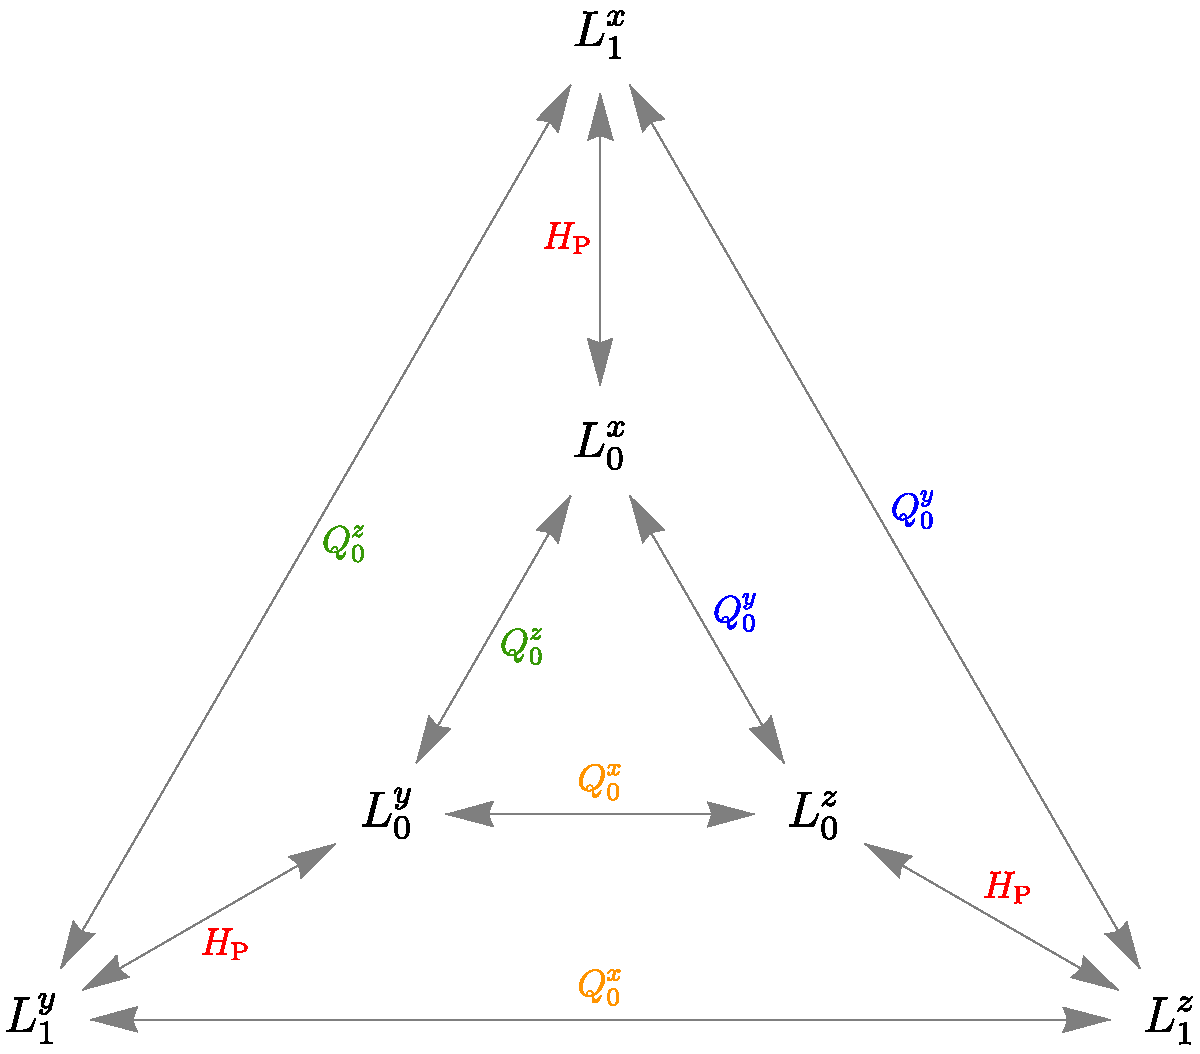
\includegraphics[width=.7\textwidth]{img/frahm_egdiagram}
\caption{A map of various eigengates between the operators $\{ L_r^\alpha \}_{r,\alpha}$ in Polychronakos' model. A quench by the operator next to an arrow implements the corresponding eigengate. }
\label{fig:polychronakos_egs}
\end{figure}
%
By noting that the eigenstates of $L_0^z$ are the computational basis states, and the commutation relations between $( L_0^\alpha, L_1^\alpha, H_P )$ are of the form of \cref{eqn:alt_comm}, we readily obtain two methods to obtain an eigengate for $L_1^z$: either by continuous evolution 
\begin{align*}
U_\text{eg}^P = \exp( -i H_\text{P} \pi / 2 ),
\end{align*}
or by adiabatically evolving $H_\text{adiabatic} = \cos( t ) L_0^z + \sin( t ) L_1^z$ for $t\in [0,\pi/2]$. Interestingly, owing to the form of $L_0^z$, applying the operation $U_\text{eg}^P$ twice performs a spatial mirror inversion and perfect state transfer on the spin chain (see \cref{sec:howtotransport}).

Another eigengate which interchanges the operator superscripts $x$, $y$ and $z$ can be formed by quenching with the total spin operator (see \cref{sec:XXXmodel})
\begin{align*}
Q_0^\beta &= \frac{1}{2} \sum_j \vec{\sigma}_j^\beta  && \beta \in \{ x,y,z \} 
\end{align*}
as it satisfies 
\begin{align*}
[ Q_0^\alpha , L_r^\beta ] &= i \epsilon^{\alpha \beta \gamma} L_r^\gamma. && r \in \{ 0, 1 \}.
\end{align*}
The different eigengates in this model are summarized in \cref{fig:polychronakos_egs}. 


\section{Resonant driving on Polychronakos eigenstates}
%
\begin{figure}[t]
\centering
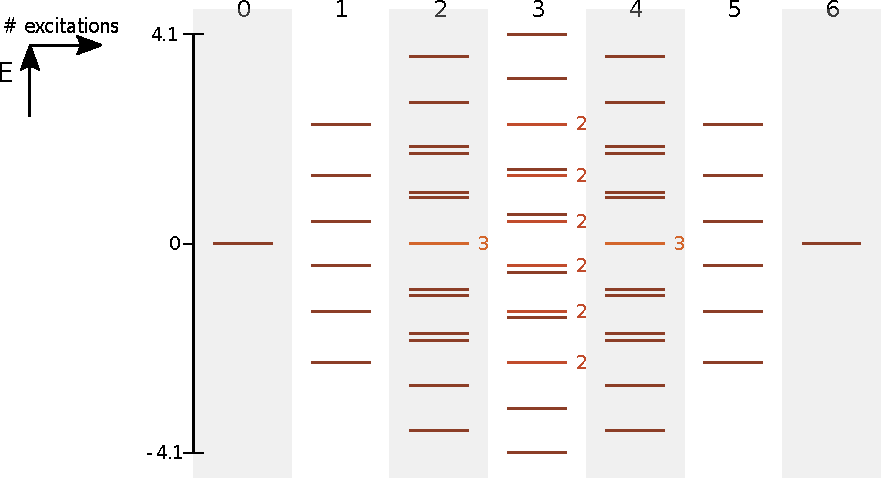
\includegraphics[width=.84\textwidth]{img/L0spectrum}
\caption{The spectrum of each of the operators $\{ L_i^\alpha \}$, depicted for $N=6$. The horizontal ordering denotes the number of $\alpha$-excitations (or Hamming weight) $\frac{N}{2} - < Q_0^\alpha>$.  Subspaces with multiplicity larger than 1 have their multiplicity displayed to their right.}
\label{fig:L0spec}
\end{figure}
%
The energy spectra of all $\{ L_r^\alpha \} $ are identical to that of $L_0^z$ as these operators are linked by an isospectral transformation. Since $H_P$ commutes with each total spin operator $\{ Q_0^\alpha \}$, we conclude that the eigensystem of each $L_i^\alpha$ separates into non-interacting blocks of constant $Q_0^\alpha$ (e.g. total spin projection in the $\alpha$ direction). From here onwards, we will focus on $\alpha = z$, but we stress that identical results hold for the $x$ and $y$ superscripts, up to a local basis transformation. 

The spectrum of $L_0^z$ for $N=6$ is depicted in \cref{fig:L0spec} with energies represented vertically and the value of $Q_0^z$ horizontally. Let $\ket{ \{ k_1, k_2, \ldots, k_p \} }$ with $k_1 < k_2 < \ldots < k_p$ represent the state with qubits $k_j$ in state $\ket{1}$ and all other qubits in the state $\ket{0}$. The energies of states expressed in this notation are conveniently calculated as 
\begin{align*}
L_0^z \ket{ \{ k_1, k_2, \ldots, k_p \} } = \sum_{j=1}^p x_{k_j} \ket{ \{ k_1, k_2, \ldots, k_p \} }.
\end{align*}
In words: for each qubit in state $\ket{1}$, add energy equal to the position $x_j$ of that qubit. 

Because the positions $x_j$ are symmetric around $0$, the highest- and lowest energy states are nondegenerate for even $N$, and are given by:
\begin{align*}
\ket{\text{high}} &= \ket{t_1} = \ket{ 0 }^{ \otimes \frac{N}{2} } \ket{ 1 }^{ \otimes \frac{N}{2} } = \ket{ \{ \frac{N}{2} + 1, \ldots, N \} } && (N \text{ even}) \\
\ket{\text{low}} &= \ket{t_2} = \ket{ 1 }^{ \otimes \frac{N}{2} } \ket{ 0 }^{ \otimes \frac{N}{2} } = \ket{ \{ 1, \ldots, \frac{N}{2} \} }
\end{align*}
As the energy gap between $\ket{t_1}$ and $\ket{t_2}$ is unique, we may select these two states for a resonantly driven multiqubit gate. However, these states are of product form in the eigenbasis, hence a local operator cannot have nonzero matrix element between $\ket{t_1}$ and $\ket{t_2}$. Therefore, we employ an eigengate $U^P_{\text{eg}}$ to turn $\ket{t_1}, \ket{t_2}$ into spatially extended states $\ket{t_1}_{L_1^z}$ and $\ket{t_2}_{L_1^z}$, while preserving the spectrum and in particular the unique energy gap. We can then resort to the driving protocol proposed in \cref{sec:resdriveprotocol} to create an $\iswap_{t_1,t_2}$ gate by choosing $H_\text{bg} = L_1^{z}$ and choosing for $H_\text{drive}$ any operator that couples $\ket{t_1}_{L_1^z}$ and $\ket{t_2}_{L_1^z}$. 

It is not clear in general what choices of $H_\text{drive}$ lead to lower gate errors at similar driving times. One constraint is that the coupling must preserve the expectation value of $Q_0^\alpha$ (i.e. the number of spins in state $\ket{1}$), indicating that couplings such as $\sigma^x$ or $\sigma^z \otimes \sigma^y$ cannot drive the required transition. For some common nontrivial 1- and 2-local driving operators and small system sizes $N$, we tabulate the matrix elements $_{L_1^z} \bra{t_1} H_\text{drive} \ket{t_2}_{L_1^z}$ below. 

{ \footnotesize 
\begin{center}
  \begin{tabular}{ | l | c | }
  	\hline
    \multicolumn{2}{ | c | }{$N=4$}  \\ \hline
	$H_\text{drive}$ 			& $ _{L_1^z} \bra{t_1} H_\text{drive} \ket{t_2}_{L_1^z} $  \\ \hline
	$\sigma^z_2$				& $-0.413049 i$ \\
    $\sigma^z_2 \sigma^z_3$ 	& $0.829345$ \\
    $\sigma^z_1 \sigma^z_4$ 	& $0.829345$ \\
   	$\sigma^x_2 \sigma^x_3$ 	& $-0.552743$ \\
	$\sigma^y_2 \sigma^y_3$ 	& $-0.552743$ \\
    $\sigma^x_1 \sigma^x_4$ 	& $0.390066$ \\
	$\sigma^x_2 \sigma^y_3$ 	& $0$ \\
	\hline
  \end{tabular}
\quad
  \begin{tabular}{ | l | c | }
  	\hline
    \multicolumn{2}{ | c | }{$N=6$}  \\ \hline
	$H_\text{drive}$ 			& $ _{L_1^z} \bra{t_1} H_\text{drive} \ket{t_2}_{L_1^z} $  \\ \hline
	$\sigma^z_3$				& $0.116012 i$ \\
    $\sigma^z_3 \sigma^z_4$ 	& $-0.327919$ \\
    $\sigma^z_1 \sigma^z_5$ 	& $-0.353636$ \\
    $\sigma^z_1 \sigma^z_5$ 	& $0.265128$ \\ 
	$\sigma^x_3 \sigma^x_4$ 	& $0.200378$ \\
	$\sigma^x_2 \sigma^x_3$ 	& $-0.147838$ \\
	$\sigma^x_1 \sigma^x_5$ 	& $-0.14341$ \\
	\hline
  \end{tabular}
\quad
  \begin{tabular}{ | l | c | }
  	\hline
    \multicolumn{2}{ | c | }{$N=8$}  \\ \hline
	$H_\text{drive}$ 			& $ _{L_1^z} \bra{t_1} H_\text{drive} \ket{t_2}_{L_1^z} $  \\ \hline
	$\sigma^z_4$				& $ -0.027894 i $ \\
    $\sigma^z_4 \sigma^z_5$ 	& $ -0.0839009 $ \\
	$\sigma^z_1 \sigma^z_6$ 	& $ 0.120287 $ \\
	$\sigma^z_2 \sigma^z_7$ 	& $ 0.131574 $ \\
	$\sigma^x_4 \sigma^x_5$ 	& $ 0.0471167 $ \\
	$\sigma^x_1 \sigma^x_6$ 	& $ 0.0502561 $ \\
	$\sigma^x_2 \sigma^x_7$ 	& $ 0.0452589 $ \\
	\hline
  \end{tabular}
\end{center}
}



\subsection{Tracking dynamical phases}
As the energies of $L_1^z$ are sums of single-excitation energies, it is possible to keep track of dynamical phases of individual states efficiently. One could in principle perform an eigengate $U^P_{eg}$, drive a transition in time $t_d$, and map back to the computational basis using $(U^P_\text{eg})^\dagger$. The accumulated dynamical phases on qubit $j$ is then equal to $x_j t_d$, which may be undone by a single-qubit phase gate, or by following the halfway inversion protocol. 




\section{Numerical results}
\label{sec:numerics}

We test our claims by simulating the driving step of our protocol, through numerically solving Schr\"{o}dinger's equation given by the Hamiltonian
\begin{align*}
H_P(t) =  L_1^z + \A_P \cos(\omega t) H_\text{drive}.
\end{align*}
We consider the cases $N=4$ and $N=6$, and two different driving operators $H_\text{drive}$ which fit in the connectivity of the linear chain. The driving frequency $\omega$ is always chosen to be exactly the energy gap between states $\ket{t_1}_{L_1^z}$ and $\ket{t_2}_{L_1^z}$. Moreover, after fixing the driving time $t_d$, we choose $\A_P$ such that a $\pi$-rotation occurs between the transitioning states, e.g. $|  _{L_1^z}\bra{t_2} H_\text{drive} \ket{t_1}_{L_1^z} | ~ \A_P ~ t_d = \pi$. Apart from the halfway inversion, we apply no further optimizations to the protocol. 

The results are presented in \cref{fig:drivefids}. For extremely short driving times, where $t_d \approx 1$ such that $\A_P$ is of the order of energy differences of the background Hamiltonian, the gate is highly inaccurate. However, for longer driving times, $t_d > 10$, the gate becomes increasingly accurate, with the error decaying roughly as $t_d^{-2}$ as expected. We also note that the fidelity seems to not strongly depend on the choice of driving operator. 

\begin{figure}[p]
\centering
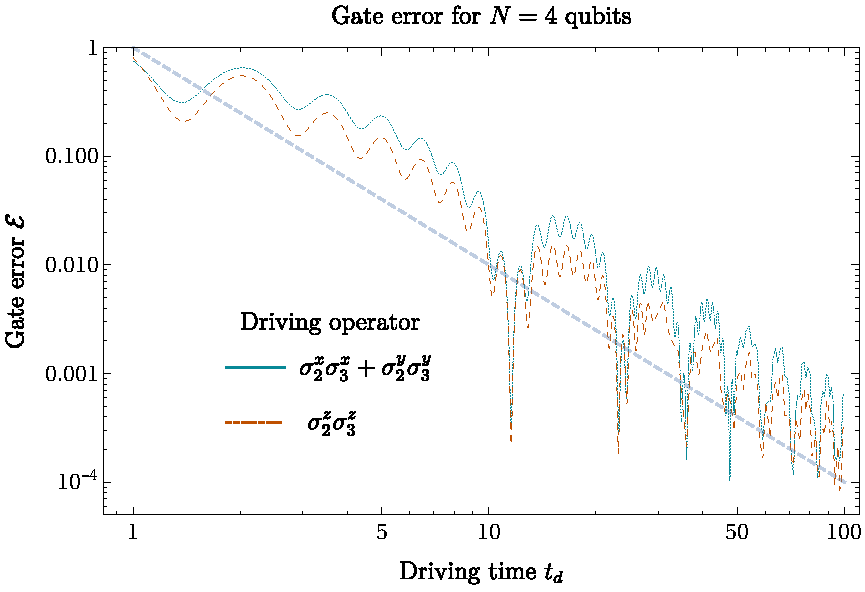
\includegraphics[width=.74\textwidth]{img/PolychronakosDriveFids4.pdf} 
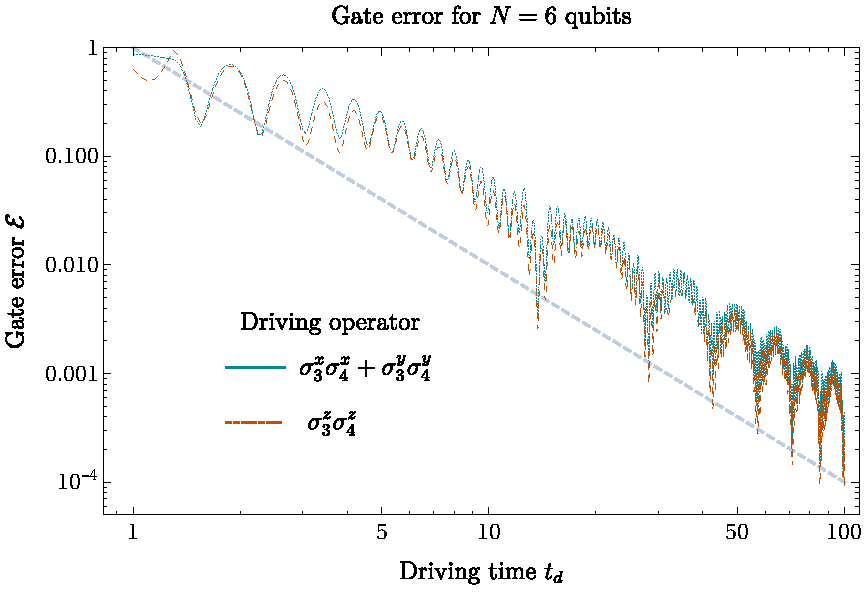
\includegraphics[width=.74\textwidth]{img/PolychronakosDriveFids6.pdf}
\caption{Gate error due to the resonant driving stage of our protocol, given various gate times and two different choices of $H_\text{drive}$, for a number of qubits equal to $N=4$ (top) and $N=6$ (bottom). In these results, we applied the halfway inversion, but no further optimizations. The dashed line follows $\mathcal{E} = t_d^{-2}$. Although the fidelity is strongly oscillatory in $t_d$, a global tendency towards inverse quadratic decay is clearly visible.} %
\label{fig:drivefids}
\end{figure}

In \cref{fig:compare_hwp}, we depict the effect of the halfway inversion compared to leaving it out. In the latter case, we undo the accumulated dynamical phases with the operation $\exp( +i L^z_0 t_d)$ after the system is mapped back to the computational basis. The graph shows that the halfway inversion does not necessarily reduce the error at all times, but dramatically improves the error at very specific times. 

We suspect that these specific times are precisely the times where, at the time of the halfway inversion, the relative phases of each two-level system are roughly $0$, causing the error's leading order term $8 \sin(nt) (\A^2 / \delta^2)$ (\cref{eqn:hwp_error}) to be minimized. We informally check this statement in \cref{fig:drivephases}, where the phases corresponding to highly optimal time $t_d = 11.55$ and local maximum $t_d = 16.55$, as well as the point precisely in between, are compared. The circles show the accumulated phase due to $H_\text{bg}$ for the indicated two-level system, with the rightmost point of the circle corresponding to zero phase. Clearly, the optimal timing is associated with near-optimal phase resets, whereas the more erroneous timing shows phases that could contribute a significant error of order $\A^2 / \delta^2$.

\begin{figure}
\centering
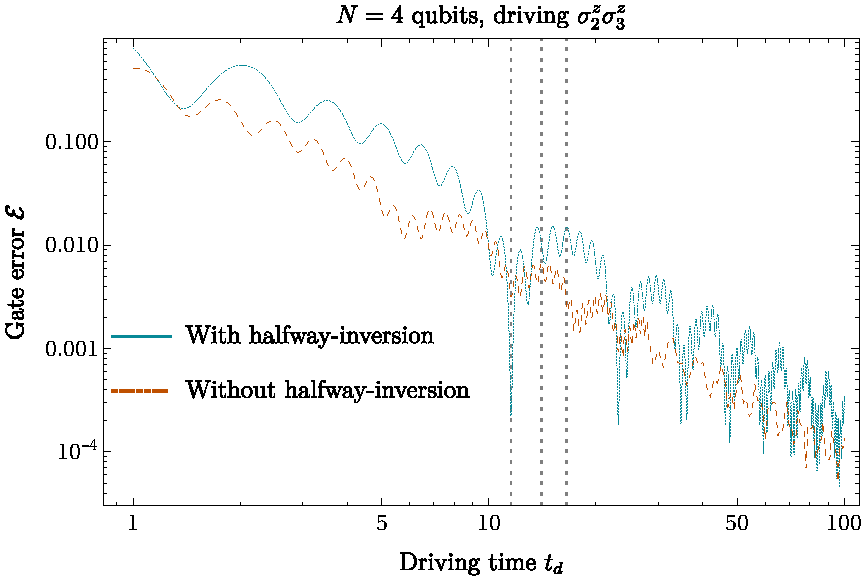
\includegraphics[width=.74\textwidth]{img/Polychronakos_compare_hwp.pdf} 
\caption{A comparison of the gate error either with or without a halfway inversion applied, for the case $N=4$ and $H_\text{drive} = \sigma_2^z \sigma_3^z$. The halfway inversion shows stronger oscillatory behavior, leading to minima that improve the total protocol fidelity by more than an order of magnitude at equal driving times. The times $t_d \in \{ 11.55, 14.05, 16.55 \}$ are highlighted with a gray, dotted line.}
\label{fig:compare_hwp}
\end{figure}



\begin{figure}
\centering
%
%
%
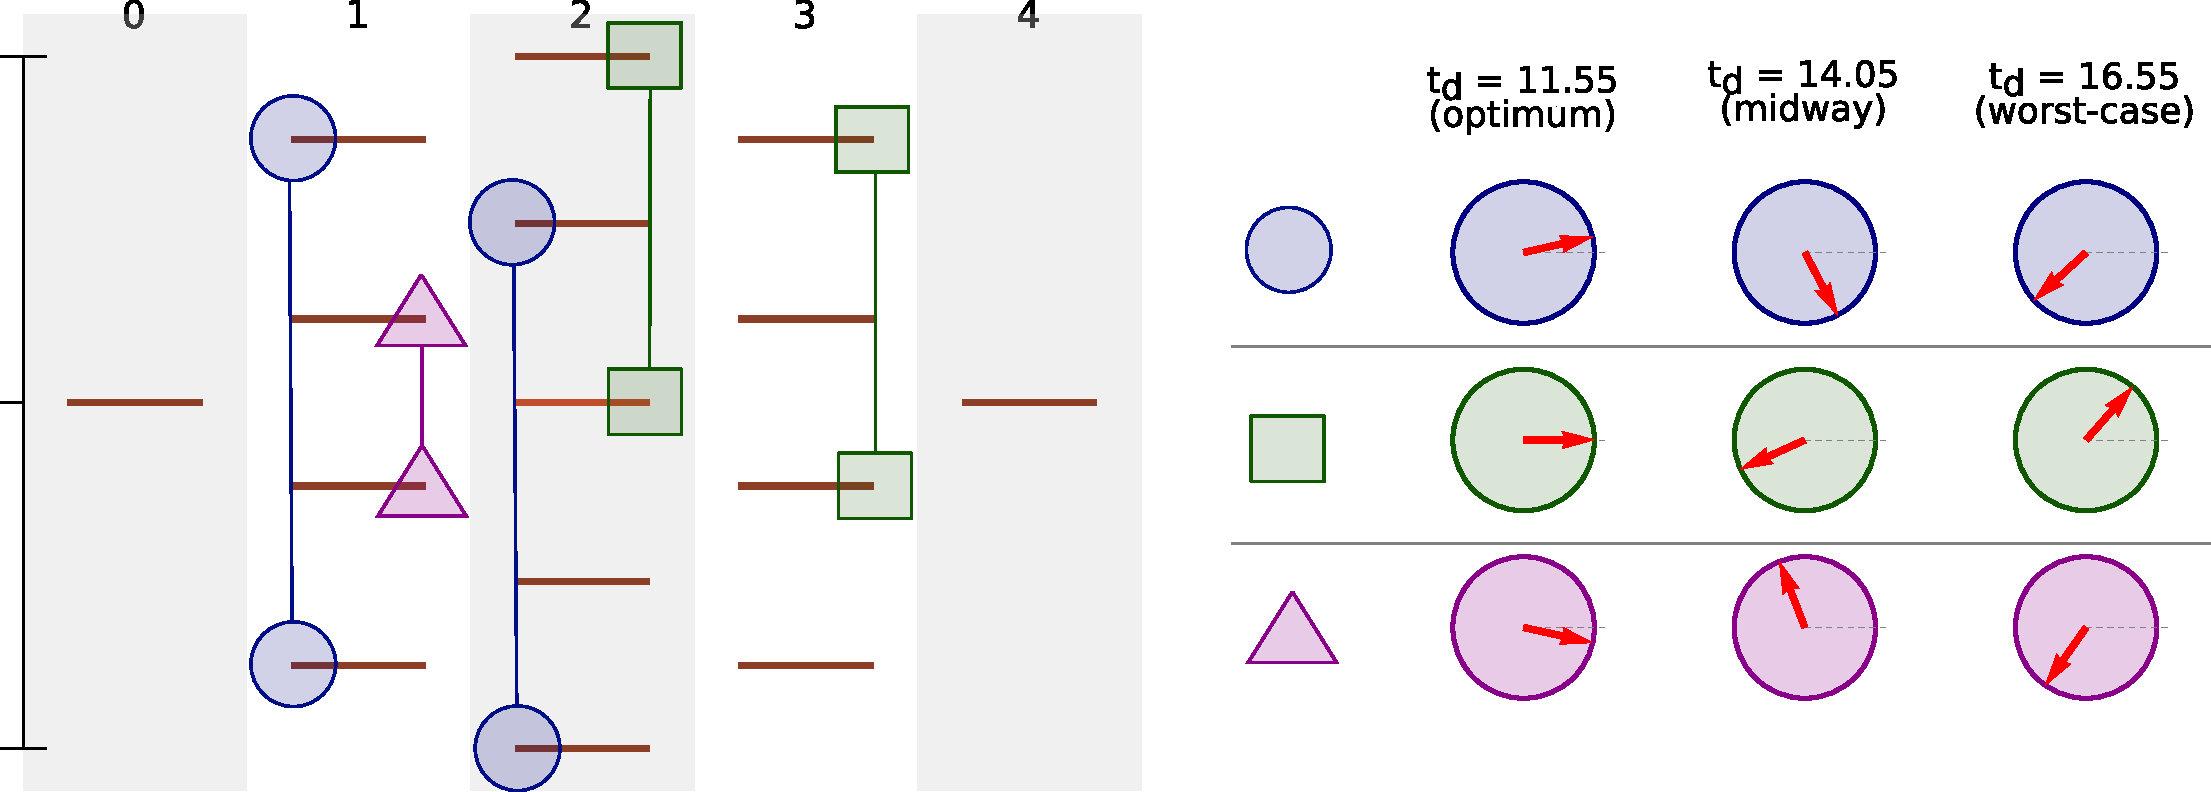
\includegraphics[width=.99\textwidth]{img/phases_goodbad.pdf}
\caption{For near-resonant two-level systems, the accumulated phases at the time of the halfway-pulse ($t_d / 2$) affect the fidelity of protocol. In the spectrum of $L_1^z$ with $N=4$ qubits, we select three different energy gaps (indicated by a pair of connected circles, squares or triangles), for which we depict the corresponding relative phases at $t_d$ as vectors on the unit sphere. A relative phase of $0$ corresponds to a vector pointing to the right (dashed lines). At $t_d = 11.55$, corresponding to a local minimum of our gate error $\mathcal{E}$, all phases are close to zero. On the other hand, at local maximum $t_d = 16.55$, the phases are all far from zero. The (non-)alignment of these phases explains the oscillatory behavior of our protocol's error as a function of time. }
\label{fig:drivephases}
\end{figure}

\subsection{Comparison of gate times}
So how do our driving times $t_d$ compare to other quantum gate times in the same system? A conventional two-qubit gate could be constructed if each of the individual Hamiltonian terms $h_{jk} P_{jk}$ could be turned on independently. A $\pi/4$ pulse would suffice to create maximal entanglement, so we require times $t$ such that $h_{jk} t = \pi / 4$. For $N=4$, the corresponding times $t$ lie between $0.86$ and $1.0$ for neighboring qubits, and up to $8.56$ for the most distant qubits. These should be compared to the $11.55$ units of time required to perform an $\iswap_{1100, 0011}$ at low  error $\mathcal{E} < 0.001$. Hence, within the time of our four-qubit $\iswap$ operation, up to $13$ two-qubit gates could be done. 

Similarly, for $N=6$, neighboring qubits could be entangled in times between $0.60$ and $0.81$, or up to $17.36$ to entangle the outermost qubits. This should be compared to the driving time $t_d = 13.75$ to obtain a driven gate with error $\mathcal{E} < 0.003$. Hence, our six-qubit resonant gate takes time equivalent to up to $23$ two-qubit gates. 

In general, it is unclear how to compare gate times between different gate sets, or how to optimally decompose $\iswap$ operations into smaller constituents. Turning to the well-studied \texttt{Toffoli} gate, the best bounds we could find are listed in Ref. \cite{Shende2009}, stating that a \texttt{Toffoli} on four qubits requires between $8$ and $14$ \texttt{CNOT} operations. Note that these results assume full connectivity between all qubits, and do not account for the cost of single-qubit gates. For larger numbers of qubits, the \texttt{CNOT} cost is found to scale linearly in $N$ as long as auxiliary qubits may be used - without auxiliaries, it would be quadratic. Different physical interactions may also lead to different gate counts. For example, Ref. \cite{Schuch2003} finds that constructing a \texttt{CNOT} out of our interaction $P_{jk}$ requires two $\pi/4$ pulses, and constructing a mere three-qubit \texttt{Toffoli} using the closely related XX interaction requires as much as ten fundamental entangling operations. We conclude that it is not possible to make a rigorous comparison between different gate sets, but that the duration of our resonantly driven gate is competitive with conventional decompositions, with both approaches having unique advantages and disadvantages depending on the specific implementation.  


\section{Conclusion}
The operators $L_0^\alpha$ and $L_1^\alpha$ turn out to be related by fast quenches of Hamiltonians such as $H_P$ and $Q_0^\alpha$. This provides a large amount of utility when these interactions are available to a system, allowing straightforward basis transformations, such as the eigengate for $L_1^z$ that we considered here. It would be interesting to look for further applications of these quenches. 

Just as with the Krawtchouk chain, the driven multiqubit gates are limited in use due to the unfavorable scaling of the matrix elements for the driving operators that we consider. In the next chapter, we discuss a system in which these numbers do not decay with system size, but this requires a star-shaped graph where many qubits are strongly coupled to a single ancilla. Finding a well-understood \emph{linear chain} that allows driven multiqubit gates even in the large $N$ limit remains an open problem.

